\cleardoublepage



\chapter{Étude de fonctionnement}

Avant de développer la solution, il est nécessaire d'étudier les besoins de la solution finale.
Chacun de ces besoins peut mettre en œuvre l'utilisation d'outils, ou peut exiger certains réglages.
\\





%%%%%%%%%%%%%%%%%%%%%%%%%%%%%%%%%%%%%%%%%%%%%%%%%%%%%%%%%%%%%%%%%%%%%%%%%%%%%%%%%%%%%%%%%%%%%%%%%%%%
%%%%%%%%%%%%%%%%%%%%%%%%%%%%%%%%%%%%%%%%%%%%%%%%%%%%%%%%%%%%%%%%%%%%%%%%%%%%%%%%%%%%%%%%%%%%%%%%%%%%
%%%%%%%%%%%%%%%%%%%%%%%%%%%%%%%%%%%%%%%%%%%%%%%%%%%%%%%%%%%%%%%%%%%%%%%%%%%%%%%%%%%%%%%%%%%%%%%%%%%%
%%%%%%%%%%%%%%%%%%%%%%%%%%%%%%%%%%%%%%%%%%%%%%%%%%%%%%%%%%%%%%%%%%%%%%%%%%%%%%%%%%%%%%%%%%%%%%%%%%%%
%%%%%%%%%%%%%%%%%%%%%%%%%%%%%%%%%%%%%%%%%%%%%%%%%%%%%%%%%%%%%%%%%%%%%%%%%%%%%%%%%%%%%%%%%%%%%%%%%%%%

\section{Construction des machines}
\label{Construction des machines}

%%%%%%%%%%%%%%%%%%%%%%%%%%%%%%%%%%%%%%%%%%%%%%%%%%%%%%%%%%%%%%%%%%%%%%%%%%%%%%%%%%%%%%%%%%%%%%%%%%%%
%%%%%%%%%%%%%%%%%%%%%%%%%%%%%%%%%%%%%%%%%%%%%%%%%%%%%%%%%%%%%%%%%%%%%%%%%%%%%%%%%%%%%%%%%%%%%%%%%%%%
%%%%%%%%%%%%%%%%%%%%%%%%%%%%%%%%%%%%%%%%%%%%%%%%%%%%%%%%%%%%%%%%%%%%%%%%%%%%%%%%%%%%%%%%%%%%%%%%%%%%

\subsection{Machine de développement}

Une première machine virtuelle, composée d'une distribution Fedora 16 64 bits, a été mise en place avec un environnement complet de développement.

Cette machine comporte toutes les bibliothèques nécessaires à la compilation des différents outils.

C'est grâce à cette machine que la solution finale sera mise en place, car elle permettra de tester les différents outils utilisés.
\\




%%%%%%%%%%%%%%%%%%%%%%%%%%%%%%%%%%%%%%%%%%%%%%%%%%%%%%%%%%%%%%%%%%%%%%%%%%%%%%%%%%%%%%%%%%%%%%%%%%%%
%%%%%%%%%%%%%%%%%%%%%%%%%%%%%%%%%%%%%%%%%%%%%%%%%%%%%%%%%%%%%%%%%%%%%%%%%%%%%%%%%%%%%%%%%%%%%%%%%%%%
%%%%%%%%%%%%%%%%%%%%%%%%%%%%%%%%%%%%%%%%%%%%%%%%%%%%%%%%%%%%%%%%%%%%%%%%%%%%%%%%%%%%%%%%%%%%%%%%%%%%

\subsection{Machine minimale}

Une seconde machine virtuelle, a été installée de façon minimale.

Elle se base sur le même système d'exploitation (Fedora 16 64 bits) pour que les différents outils compilés sur la machine virtuelle "complète" soient compatibles avec la machine virtuelle "minimale".

Les avantages d'un système d'exploitation minimal, sont :
\begin{itemize}
	\item démarrage et arrêt plus rapide : Lors du démarrage le système démarre les différents services qui mettent un certain temps à s'exécuter. Ici, seuls les services vitaux et ceux que l'on utilisera seront démarrés. De plus, lors de l'extinction le système aura moins de processus à arrêter.
	\item système moins "lourd" : Lorsque le système est en marche, de nombreux processus sont lancés, et utilisent des ressources (CPU et RAM).
	\item absence d'interface graphique : Le serveur X qui permet l'affichage des différentes fenêtres graphiques consomme aussi des ressources.
	\item taille minimale : Seuls les programmes indispensables sont installés, ce qui permet d'avoir une installation minimale (200Mo au lieu des 4Go).
\\
\end{itemize}

% init 3
Cette machine n'est contrôlable uniquement en ligne de commande, ce qui est assez compliqué pour effectuer les différents tests.
On utilisera donc cette machine virtuelle une fois la solution fonctionnelle.
\\





%%%%%%%%%%%%%%%%%%%%%%%%%%%%%%%%%%%%%%%%%%%%%%%%%%%%%%%%%%%%%%%%%%%%%%%%%%%%%%%%%%%%%%%%%%%%%%%%%%%%
%%%%%%%%%%%%%%%%%%%%%%%%%%%%%%%%%%%%%%%%%%%%%%%%%%%%%%%%%%%%%%%%%%%%%%%%%%%%%%%%%%%%%%%%%%%%%%%%%%%%
%%%%%%%%%%%%%%%%%%%%%%%%%%%%%%%%%%%%%%%%%%%%%%%%%%%%%%%%%%%%%%%%%%%%%%%%%%%%%%%%%%%%%%%%%%%%%%%%%%%%
%%%%%%%%%%%%%%%%%%%%%%%%%%%%%%%%%%%%%%%%%%%%%%%%%%%%%%%%%%%%%%%%%%%%%%%%%%%%%%%%%%%%%%%%%%%%%%%%%%%%
%%%%%%%%%%%%%%%%%%%%%%%%%%%%%%%%%%%%%%%%%%%%%%%%%%%%%%%%%%%%%%%%%%%%%%%%%%%%%%%%%%%%%%%%%%%%%%%%%%%%

\section{Paramétrisation de la machine virtuelle}
\label{Paramétrisation de la machine virtuelle}

\begin{figure}[!h]
	\center
	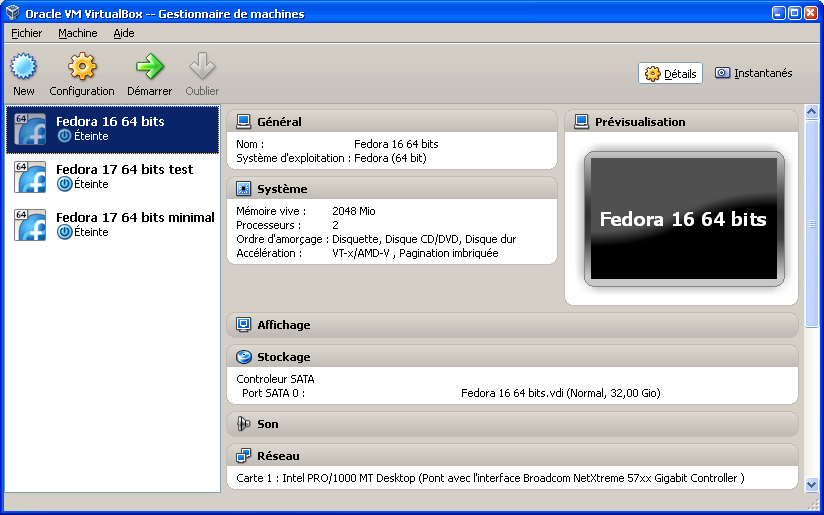
\includegraphics[scale=0.5]{images/VirtualBox.png}
	\caption{Interface graphique de VirtualBox}
	\label{Interface graphique de VirtualBox}
\end{figure}

VirtualBox dispose d'une interface graphique, présente sur la capture d'écran \ref{Interface graphique de VirtualBox}, qui permet de paramétrer facilement l'ensemble des machines virtuelles.

Cette interface possède toutefois quelques limites, car lorsque la machine virtuelle est allumée, il est impossible de modifier la majorité de ses paramètres.
\\


L'objectif du projet est de fournir une solution de virtualisation simple, qui permettrait d'effectuer des calculs scientifiques de manière automatique.
Il faut donc trouver une solution efficace qui permettrait de paramétrer automatiquement l'interface graphique, pour que l'utilisateur n'ait pas à le faire.
\\




%%%%%%%%%%%%%%%%%%%%%%%%%%%%%%%%%%%%%%%%%%%%%%%%%%%%%%%%%%%%%%%%%%%%%%%%%%%%%%%%%%%%%%%%%%%%%%%%%%%%
%%%%%%%%%%%%%%%%%%%%%%%%%%%%%%%%%%%%%%%%%%%%%%%%%%%%%%%%%%%%%%%%%%%%%%%%%%%%%%%%%%%%%%%%%%%%%%%%%%%%
%%%%%%%%%%%%%%%%%%%%%%%%%%%%%%%%%%%%%%%%%%%%%%%%%%%%%%%%%%%%%%%%%%%%%%%%%%%%%%%%%%%%%%%%%%%%%%%%%%%%

\subsection{LibVirt}

L'utilisation de deux types différents de machine virtuelle (VirtualBox et VMware) dans l'entreprise Hutchinson impose le développement d'une solution compatible avec chacune d'elles.
\\


\textit{LibVirt}\footnote{LibVirt - Site web : http://libvirt.org} est une API\footnote{API (Application Programming Interface) : ensemble de fonctions mises à disposition par une bibliothèque logicielle, permettant l'interaction entre les différents programmes.} de gestion de virtualisation, qui permet de contrôler de nombreuses plateformes de virtualisation, telles que :
\begin{itemize}
	\item VirtualBox ;
	\item QEMU ;
	\item VMware \ldots
\end{itemize}

C'est une bibliothèque open-source, codée en Langage C et développée par la société \href{http://http://www.redhat.com}{Red Hat}, qui utilise une couche d'abstraction pour être compatible avec chacune d'entre elles.
\\


Initialement prévue pour être utilisée sur une plateforme Unix/Linux, il serait possible de l'installer et l'utiliser sur les différents systèmes d'exploitation, dont Windows, en effectuant quelques manipulations.
La première méthode consiste à compiler la bibliothèque avec MinGW, qui est un émulateur de terminal Linux qui permet la compilation de programmes Linux en exécutables Windows.
Rencontrant plusieurs problèmes, notamment en raison de problèmes de certificats de sécurité, cette première méthode n'a pu aboutir.

La seconde méthode a pour objectif de cross-compiler LibVirt. Cela consiste à compiler la bibliothèque sous Linux, en spécifiant certaines options lors de la compilation, pour pouvoir être exporté sur un système d'exploitation différent. Dans le cas de l'exportation de Linux vers Windows, la compilation produira des exécutables (d'extension \textit{.exe}) et des bibliothèques dynamiques (d'extension \textit{.dll}). A la suite de cette cross-compilation les fichiers générés seraient directement exécutables sous Windows. 
Cette méthode a été concluante car il était bien possible d'utiliser LibVirt dans des scripts Python, mais la connexion avec la machine virtuelle était impossible pour des raisons inconnues.
\\




%%%%%%%%%%%%%%%%%%%%%%%%%%%%%%%%%%%%%%%%%%%%%%%%%%%%%%%%%%%%%%%%%%%%%%%%%%%%%%%%%%%%%%%%%%%%%%%%%%%%
%%%%%%%%%%%%%%%%%%%%%%%%%%%%%%%%%%%%%%%%%%%%%%%%%%%%%%%%%%%%%%%%%%%%%%%%%%%%%%%%%%%%%%%%%%%%%%%%%%%%
%%%%%%%%%%%%%%%%%%%%%%%%%%%%%%%%%%%%%%%%%%%%%%%%%%%%%%%%%%%%%%%%%%%%%%%%%%%%%%%%%%%%%%%%%%%%%%%%%%%%

\subsection{VBoxManage}
\label{VBoxManage}

Suite à l'incapacité d'utiliser la bibliothèque LibVirt, il fallait donc trouver une autre technique pour contrôler la machine virtuelle.
\\


VirtualBox propose, en plus de l'interface graphique présentée en début de la partie \ref{Paramétrisation de la machine virtuelle}, un programme en ligne de commande : \lstinline{VBoxManage}.
Il propose la configuration des machines virtuelles (nombre de cœurs et RAM allouée, \ldots), mais aussi la manipulation et l'affichage d'informations des disques virtuels, des répertoires partagés, \ldots

Ce programme est installé en même temps que le logiciel VirtualBox, et peut être directement utilisé dans les terminaux de la machine hôte.
\\




%%%%%%%%%%%%%%%%%%%%%%%%%%%%%%%%%%%%%%%%%%%%%%%%%%%%%%%%%%%%%%%%%%%%%%%%%%%%%%%%%%%%%%%%%%%%%%%%%%%%
%%%%%%%%%%%%%%%%%%%%%%%%%%%%%%%%%%%%%%%%%%%%%%%%%%%%%%%%%%%%%%%%%%%%%%%%%%%%%%%%%%%%%%%%%%%%%%%%%%%%
%%%%%%%%%%%%%%%%%%%%%%%%%%%%%%%%%%%%%%%%%%%%%%%%%%%%%%%%%%%%%%%%%%%%%%%%%%%%%%%%%%%%%%%%%%%%%%%%%%%%

\subsection{VirtualBox SDK}

VirtualBox propose un SDK\footnote{SDK (Software Development Kit) : ensemble d'outils mis à la disposition des développeurs, permettant la création d'application.} permettant aussi un contrôle des machines virtuelles.
Cette API propose plusieurs classes, programmées dans plusieurs langages : C++ et Python.

Contrairement à VBoxManage, ce SDK n'est pas installé avec VirtualBox.
Il faut donc télécharger\footnote{SDK VirtualBox - Source : \href{https://www.virtualbox.org/wiki/Downloads}{https://www.virtualbox.org/wiki/Downloads}} puis l'intégrer à la solution.
\\




%%%%%%%%%%%%%%%%%%%%%%%%%%%%%%%%%%%%%%%%%%%%%%%%%%%%%%%%%%%%%%%%%%%%%%%%%%%%%%%%%%%%%%%%%%%%%%%%%%%%
%%%%%%%%%%%%%%%%%%%%%%%%%%%%%%%%%%%%%%%%%%%%%%%%%%%%%%%%%%%%%%%%%%%%%%%%%%%%%%%%%%%%%%%%%%%%%%%%%%%%
%%%%%%%%%%%%%%%%%%%%%%%%%%%%%%%%%%%%%%%%%%%%%%%%%%%%%%%%%%%%%%%%%%%%%%%%%%%%%%%%%%%%%%%%%%%%%%%%%%%%

\subsection{Méthode choisie}

Ne réussissant pas à utiliser LibVirt, la solution devra se résoudre aux machines virtuelles de type VirtualBox.

Pour développer ma première solution, j'utiliserai VBoxManage, qui permet un contrôle simple et efficace des machines virtuelles en ligne de commande.
L'API pourrait être utilisée dans une version future, pour optimiser ou compléter la première solution.
\\





%%%%%%%%%%%%%%%%%%%%%%%%%%%%%%%%%%%%%%%%%%%%%%%%%%%%%%%%%%%%%%%%%%%%%%%%%%%%%%%%%%%%%%%%%%%%%%%%%%%%
%%%%%%%%%%%%%%%%%%%%%%%%%%%%%%%%%%%%%%%%%%%%%%%%%%%%%%%%%%%%%%%%%%%%%%%%%%%%%%%%%%%%%%%%%%%%%%%%%%%%
%%%%%%%%%%%%%%%%%%%%%%%%%%%%%%%%%%%%%%%%%%%%%%%%%%%%%%%%%%%%%%%%%%%%%%%%%%%%%%%%%%%%%%%%%%%%%%%%%%%%
%%%%%%%%%%%%%%%%%%%%%%%%%%%%%%%%%%%%%%%%%%%%%%%%%%%%%%%%%%%%%%%%%%%%%%%%%%%%%%%%%%%%%%%%%%%%%%%%%%%%
%%%%%%%%%%%%%%%%%%%%%%%%%%%%%%%%%%%%%%%%%%%%%%%%%%%%%%%%%%%%%%%%%%%%%%%%%%%%%%%%%%%%%%%%%%%%%%%%%%%%

\section{Contrôle de la machine virtuelle}
\label{Contrôle de la machine virtuelle}

%%%%%%%%%%%%%%%%%%%%%%%%%%%%%%%%%%%%%%%%

\subsection{Nécessité de communiquer avec la machine virtuelle}

Le programme VBoxManage ne permet que de paramétrer la machine virtuelle (nombre de cœurs alloués, quantité de RAM, manipulation de disques virtuels, \ldots), mais ne permet aucune action à l'intérieur du système d'exploitation virtualisé.
Par exemple, il est impossible d'accéder à l'arborescence des fichiers, de manipuler les répertoires, d'exécuter un outil installé dans la machine virtuelle, \ldots
\\




%%%%%%%%%%%%%%%%%%%%%%%%%%%%%%%%%%%%%%%%%%%%%%%%%%%%%%%%%%%%%%%%%%%%%%%%%%%%%%%%%%%%%%%%%%%%%%%%%%%%
%%%%%%%%%%%%%%%%%%%%%%%%%%%%%%%%%%%%%%%%%%%%%%%%%%%%%%%%%%%%%%%%%%%%%%%%%%%%%%%%%%%%%%%%%%%%%%%%%%%%
%%%%%%%%%%%%%%%%%%%%%%%%%%%%%%%%%%%%%%%%%%%%%%%%%%%%%%%%%%%%%%%%%%%%%%%%%%%%%%%%%%%%%%%%%%%%%%%%%%%%

\subsection{Configuration de la machine hôte}

%%%%%%%%%%%%%%%%%%%%%%%%%%%%%%%%%%%%%%%%%%%%%%%%%%%%%%%%%%%%%%%%%%%%%%%%%%%%%%%%%%%%%%%%%%%%%%%%%%%%

\subsubsection{PuTTY}
\label{PuTTY}

\textit{PuTTY}\footnote{PuTTy - Site web : \href{http://www.chiark.greenend.org.uk/~sgtatham/putty}{http://www.chiark.greenend.org.uk/$\sim$sgtatham/putty}} est un client SSH, gratuit et open-source, initialement développé pour Windows mais portable sur Linux, qui propose aussi d'autres protocoles de communication tels que Telnet, TCP ou Rlogin.
Il possède une interface graphique qui facilite la configuration du logiciel avant la connexion.

PuTTY est très utilisés sous Windows car il dispose de nombreuses fonctionnalités.
De plus, il est installé sur tous les ordinateurs du service d'Hutchinson, ce qui permet de ne pas devoir installer de logiciels supplémentaires pour déployer la solution de virtualisation.
\\



%%%%%%%%%%%%%%%%%%%%%%%%%%%%%%%%%%%%%%%%%%%%%%%%%%%%%%%%%%%%%%%%%%%%%%%%%%%%%%%%%%%%%%%%%%%%%%%%%%%%

\subsubsection{PLink}
\label{PLink}

PuTTY propose de nombreux outils liés à la communication par protocole SSH, dont PLink (PuTTY Link).
Il s'agit d'un client SSH, Telnet et Rlogin, exécutable en ligne de commande, qui permet de se connecter sur un serveur distant, ou d'y lancer des commandes à distance.
\\




%%%%%%%%%%%%%%%%%%%%%%%%%%%%%%%%%%%%%%%%%%%%%%%%%%%%%%%%%%%%%%%%%%%%%%%%%%%%%%%%%%%%%%%%%%%%%%%%%%%%
%%%%%%%%%%%%%%%%%%%%%%%%%%%%%%%%%%%%%%%%%%%%%%%%%%%%%%%%%%%%%%%%%%%%%%%%%%%%%%%%%%%%%%%%%%%%%%%%%%%%
%%%%%%%%%%%%%%%%%%%%%%%%%%%%%%%%%%%%%%%%%%%%%%%%%%%%%%%%%%%%%%%%%%%%%%%%%%%%%%%%%%%%%%%%%%%%%%%%%%%%

\subsection{Configuration de la machine virtuelle}
\label{Contrôle - Configuration machine virtuelle}

%%%%%%%%%%%%%%%%%%%%%%%%%%%%%%%%%%%%%%%%%%%%%%%%%%%%%%%%%%%%%%%%%%%%%%%%%%%%%%%%%%%%%%%%%%%%%%%%%%%%

\subsubsection{Serveur SSH}
\label{Serveur SSH}

Il est tout d'abord nécessaire d'installer un serveur SSH sur la machine virtuelle, pour permettre la communication entre la machine hôte et la machine virtuelle, plus précisément entre le client (PLink installé sur la machine hôte) et le serveur (installé dans la machine virtuelle).
\\


\textit{OpenSSH} est un logiciel libre et open-source, fournissant un ensemble d'outils liés à la communication par protocole SSH.
Il s'installe facilement en utilisant le gestionnaire de paquet (expliqué plus tard dans la partie \ref{L'installation}) disponible sur Linux, \lstinline{yum} ou \lstinline{apt-get} selon la distribution utilisée :
\begin{lstlisting}[language = sh]
# yum install openssh-server
# apt-get install openssh-server 
\end{lstlisting}
Une fois installé le démon (expliqué en annexe dans la partie \ref{Le service "network"}) SSH (sshd) se lancera automatiquement à chaque démarrage de la machine virtuelle.
\\



%%%%%%%%%%%%%%%%%%%%%%%%%%%%%%%%%%%%%%%%%%%%%%%%%%%%%%%%%%%%%%%%%%%%%%%%%%%%%%%%%%%%%%%%%%%%%%%%%%%%

\subsubsection{Droits administrateur}

La manipulation de la machine virtuelle impose d'effectuer des actions "critiques" au sein du système d'exploitation Linux, comme par exemple le montage et démontage de disques (commandes \lstinline{mount} et \lstinline{umount}), la création et suppression de répertoires ou fichiers (commande \lstinline{mkdir} et \lstinline{rm}).
Par défaut, les utilisateurs enregistrés sur Linux ne possèdent pas les droits administrateur, pour des raisons de sécurité, et ne peuvent pas exécuter ces commandes ou leur applications sont limitées.
\\


La commande \lstinline{sudo} (Subsitute User DO) permet aux utilisateurs, autorisés par l'administrateur, de lancer certaines commandes en tant que super-utilisateur\footnote{Super-utilisateur (ou root) : utilisateur qui possède toutes les permissions.} :
\begin{lstlisting}[language = sh]
$ sudo commande
\end{lstlisting}

Pour autoriser un utilisateur à exécuter ces commandes l'administrateur système doit lui ajouter les privilèges.
Pour cela il doit modifier le fichier de configuration \lstinline{/etc/sudoers}, et ajouter la ligne suivante :
\begin{lstlisting}
username  ALL=cmd1, cmd2, NOPASSWD: cmd3, cmd4
\end{lstlisting}
où
\begin{itemize}
	\item[username] est le nom de l'utilisateur qui recevra les droits
	\item[cmd1 et cmd2] sont les commandes qui pourront être exécutées par l'utilisateur. Il est possible d'autoriser toutes les commandes en spécifiant \lstinline{(ALL)}
	\item[cmd3 et cmd4] sont les commandes qui ne nécessiteront pas du mot de passe de l'utilisateur. Il est aussi possible d'ignorer la demande du mot de passe pour toutes les commandes en spécifiant \lstinline{(ALL)}.
\end{itemize}

Ainsi pour autoriser l'utilisateur à exécuter toutes les commandes en tant que super-utilisateur sans demande de mot de passe, il suffit d'entrer la ligne :
\begin{lstlisting}
username  ALL=(ALL) NOPASSWD: ALL
\end{lstlisting}

Notons que la modification du fichier \lstinline{/etc/sudoers} soit s'effectuer grâce à la commande \lstinline{visudo} qui permet une vérification du fichier avant enregistrement et le chargement des nouveaux paramètres dans le système.
~~\\


Enfin, une option est à désactiver dans le fichier \lstinline{/etc/sudoers} :
\begin{lstlisting}
Defaults requiretty
\end{lstlisting}
Si cette option n'est pas désactivée, les requêtes envoyées par PLink n'aboutiront pas, et retourneront un message d'erreur :
\begin{lstlisting}
sudo: sorry, you must have a tty to run sudo
\end{lstlisting}
Une fois désactivée, par exemple en commentant la ligne avec un "\#", il est possible d'utiliser la commande \lstinline{sudo} à partir d'un ordinateur distant et sans demande de mot de passe.
\\



%%%%%%%%%%%%%%%%%%%%%%%%%%%%%%%%%%%%%%%%%%%%%%%%%%%%%%%%%%%%%%%%%%%%%%%%%%%%%%%%%%%%%%%%%%%%%%%%%%%%

\subsubsection{La carte réseau}

Pour pouvoir communiquer directement avec la machine virtuelle il est nécessaire de paramétrer le réseau dans le type "Accès par pont", comme expliqué dans la partie \ref{Les types de réseau}.
Ainsi la machine virtuelle possèdera sa propre adresse IP et pourra être accessible via l'outil PLink.
\\


Il est nécessaire de connaitre l'adresse IP de la machine virtuelle pour y envoyer des commandes.
L'adressage IP sera donc réglé en "IP statique" avec une adresse IP spécifique plutôt qu'en "IP dynamique", pour ne pas avoir à retrouver l'IP après chaque démarrage de la machine virtuelle.
\\




%%%%%%%%%%%%%%%%%%%%%%%%%%%%%%%%%%%%%%%%%%%%%%%%%%%%%%%%%%%%%%%%%%%%%%%%%%%%%%%%%%%%%%%%%%%%%%%%%%%%
%%%%%%%%%%%%%%%%%%%%%%%%%%%%%%%%%%%%%%%%%%%%%%%%%%%%%%%%%%%%%%%%%%%%%%%%%%%%%%%%%%%%%%%%%%%%%%%%%%%%
%%%%%%%%%%%%%%%%%%%%%%%%%%%%%%%%%%%%%%%%%%%%%%%%%%%%%%%%%%%%%%%%%%%%%%%%%%%%%%%%%%%%%%%%%%%%%%%%%%%%

\subsection{Utilisation de PLink}
\label{Utilisation de PLink}

PLink s'exécute en ligne de commande, et requiert de spécifier les options de connexion au serveur cible :
\begin{lstlisting}[language = sh]
plink <options> "<command>"
plink -ssh -l <username> -pw <password> <IP> "<command>"
\end{lstlisting}
Après exécution de la commande, le serveur cible renvoie au client l'affichage de retour de la commande.
\\


Ce mode de communication est très efficace, mais a une latence assez élevée.
En effet, il faut environ 1/2 seconde au minimum pour envoyer une simple commande au serveur.
Donc lorsqu'il s'agit d'exécuter un grand nombre de commandes, l'envoi des commandes les unes après les autres peut durer un certain temps.

La solution consiste à envoyer plusieurs commandes simultanément au serveur, en les séparant par des ";".
Elles seront exécutées les unes à la suite des autres, et l'affichage de chacune des commandes sera retourné :
\begin{lstlisting}[language = sh]
plink <options> "<command1> ; <command2> ; <command3>"
\end{lstlisting}
Ainsi, l'envoi d'un programme Bash\footnote{Bash (Bourne-Again SHell) : shell du projet GNU, qui est l'interpréteur permettant d'exécuter des commandes.} permettra d'exécuter un mini-programme (avec tests et conditions) sur la machine virtuelle.
\\





%%%%%%%%%%%%%%%%%%%%%%%%%%%%%%%%%%%%%%%%%%%%%%%%%%%%%%%%%%%%%%%%%%%%%%%%%%%%%%%%%%%%%%%%%%%%%%%%%%%%
%%%%%%%%%%%%%%%%%%%%%%%%%%%%%%%%%%%%%%%%%%%%%%%%%%%%%%%%%%%%%%%%%%%%%%%%%%%%%%%%%%%%%%%%%%%%%%%%%%%%
%%%%%%%%%%%%%%%%%%%%%%%%%%%%%%%%%%%%%%%%%%%%%%%%%%%%%%%%%%%%%%%%%%%%%%%%%%%%%%%%%%%%%%%%%%%%%%%%%%%%
%%%%%%%%%%%%%%%%%%%%%%%%%%%%%%%%%%%%%%%%%%%%%%%%%%%%%%%%%%%%%%%%%%%%%%%%%%%%%%%%%%%%%%%%%%%%%%%%%%%%
%%%%%%%%%%%%%%%%%%%%%%%%%%%%%%%%%%%%%%%%%%%%%%%%%%%%%%%%%%%%%%%%%%%%%%%%%%%%%%%%%%%%%%%%%%%%%%%%%%%%

\section{Les échanges de fichiers}
\label{Les échanges de fichiers}

Une des nécessités dont doit se doter la solution, est la possibilité d'échange de fichiers entre la machine hôte (Windows) et la machine virtuelle (Linux).
En effet, pour pouvoir effectuer des calculs, les outils doivent disposer d'un fichier d'entrée, et vont générer des fichiers de sortie.
Il faut donc pouvoir envoyer le fichier d'entrée, puis récupérer les fichiers de sortie.
\\




%%%%%%%%%%%%%%%%%%%%%%%%%%%%%%%%%%%%%%%%%%%%%%%%%%%%%%%%%%%%%%%%%%%%%%%%%%%%%%%%%%%%%%%%%%%%%%%%%%%%
%%%%%%%%%%%%%%%%%%%%%%%%%%%%%%%%%%%%%%%%%%%%%%%%%%%%%%%%%%%%%%%%%%%%%%%%%%%%%%%%%%%%%%%%%%%%%%%%%%%%
%%%%%%%%%%%%%%%%%%%%%%%%%%%%%%%%%%%%%%%%%%%%%%%%%%%%%%%%%%%%%%%%%%%%%%%%%%%%%%%%%%%%%%%%%%%%%%%%%%%%

\subsection{Le répertoire partagé}

Cette méthode utilise la fonction du répertoire partagé : accéder aux fichiers de la machine hôte à partir de la machine virtuelle.
\\



%%%%%%%%%%%%%%%%%%%%%%%%%%%%%%%%%%%%%%%%%%%%%%%%%%%%%%%%%%%%%%%%%%%%%%%%%%%%%%%%%%%%%%%%%%%%%%%%%%%%

\subsubsection{Partager un répertoire}

Le partage d'un répertoire peut s'effectuer en utilisant l'interface graphique proposée par VirtualBox, mais est aussi possible en ligne de commande en utilisant le programme VBoxManage :
\begin{lstlisting}[language = sh]
vboxmanage sharedfolder add <VM_NAME> --name <LABEL>
                          --hostpath <PATH>
\end{lstlisting}
où 
\begin{itemize}
	\item[<VM\_NAME> :] est le nom de la machine virtuelle avec qui l'on souhaite partager le répertoire,
	\item[<LABEL> :] est le nom unique qui sera utilisé pour identifier le répertoire partagé,
	\item[<PATH> :] est le chemin du répertoire, de la machine hôte, que l'on souhaite partager.
\\
\end{itemize}


Ensuite il est nécessaire de monter le répertoire dans la machine virtuelle, pour qu'il soit accessible dans l'arborescence Linux.
Contrairement aux périphériques, le répertoire partagé n'est pas représenté par un fichier (explications faites dans la partie \ref{Les périphériques sous Linux}).
Cela s'effectue donc en utilisant son \textit{label} :
\begin{lstlisting}[language = sh]
# mount -t vboxsf <LABEL> <REP_MONT>
# mount.vboxsf <LABEL> <REP_MONT>
\end{lstlisting}
où \lstinline{mount.vboxsf} est un alias pour \lstinline{mount -t vboxsf}.
~~\\



%%%%%%%%%%%%%%%%%%%%%%%%%%%%%%%%%%%%%%%%%%%%%%%%%%%%%%%%%%%%%%%%%%%%%%%%%%%%%%%%%%%%%%%%%%%%%%%%%%%%

\subsubsection{Principe de l'échange}
\label{Principe de l'échange par répertoire partagé}

\paragraph{L'émission :}
Prenons l'exemple d'un fichier source \lstinline{C:\chemin...source\fichier.txt} que l'on souhaite envoyer vers le répertoire \lstinline{/chemin...cible/repertoire/} :
\begin{enumerate}
	\item on partage le répertoire parent de la cible avec la machine virtuelle : \lstinline{C:\chemin...source\}
	\item on monte le répertoire partagé dans la machine virtuelle, à un endroit "quelconque", par exemple : \lstinline{/media/}
	\item on effectue (dans la machine virtuelle) la copie du fichier \lstinline{/media/fichier.txt} vers le répertoire cible \lstinline{/chemin...cible/repertoire/}
	\item on démonte le répertoire partagé (optionnel)
\end{enumerate}
Cette méthode fonctionne aussi pour l'envoyer d'un répertoire.
\\


\paragraph{La réception :}
Pour recevoir un fichier \lstinline{/chemin...source/fichier.txt} vers le répertoire \lstinline{C:\chemin...cible\}, la méthode est quasiment la même :
\begin{enumerate}
	\item on partage le répertoire cible avec la machine virtuelle : \lstinline{C:\chemin...cible\}
	\item on monte le répertoire partagé dans la machine virtuelle, à un endroit "quelconque", par exemple : \lstinline{/media/}
	\item on effectue (dans la machine virtuelle) la copie du fichier \lstinline{/chemin...source/fichier.txt} versle répertoire cible \lstinline{/media/}
	\item on démonte le répertoire partagé (optionnel)
\end{enumerate}
Cette méthode fonctionne aussi pour la réception d'un répertoire.
\\




%%%%%%%%%%%%%%%%%%%%%%%%%%%%%%%%%%%%%%%%%%%%%%%%%%%%%%%%%%%%%%%%%%%%%%%%%%%%%%%%%%%%%%%%%%%%%%%%%%%%
%%%%%%%%%%%%%%%%%%%%%%%%%%%%%%%%%%%%%%%%%%%%%%%%%%%%%%%%%%%%%%%%%%%%%%%%%%%%%%%%%%%%%%%%%%%%%%%%%%%%
%%%%%%%%%%%%%%%%%%%%%%%%%%%%%%%%%%%%%%%%%%%%%%%%%%%%%%%%%%%%%%%%%%%%%%%%%%%%%%%%%%%%%%%%%%%%%%%%%%%%

\subsection{SSH}
\label{Échange par SSH}

Le protocole SSH permet, en plus de l'envoi de commande, d'échanger des fichiers très simplement en ligne de commande, et de façon sécurisée.
\\



%%%%%%%%%%%%%%%%%%%%%%%%%%%%%%%%%%%%%%%%%%%%%%%%%%%%%%%%%%%%%%%%%%%%%%%%%%%%%%%%%%%%%%%%%%%%%%%%%%%%

\subsubsection{Configuration de la machine hôte}

PuTTY propose un autre outil, disponible aussi en ligne de commande, qui permet l'échange de fichier avec un serveur distant : \textit{Pscp} (PuTTY Secure Copy).
Il est, comme PLink, installé par défaut avec le logiciel PuTTY (confère partie \ref{PLink} pour plus de détails).
Ce programme s'exécute en ligne de commande, et permet l'utilisation de différents protocoles d'échange : SSH, FTP, \ldots
\\



%%%%%%%%%%%%%%%%%%%%%%%%%%%%%%%%%%%%%%%%%%%%%%%%%%%%%%%%%%%%%%%%%%%%%%%%%%%%%%%%%%%%%%%%%%%%%%%%%%%%

\subsubsection{Configuration de la machine virtuelle}

La machine virtuelle doit disposer d'un serveur SSH pour que le client (Plink) s'y connecte.
La configuration sera exactement la même que celle utilisée pour l'envoi de commande, développée dans la partie \ref{Contrôle - Configuration machine virtuelle}.
Aucune configuration supplémentaire ne sera donc nécessaire pour permettre l'échange de fichiers.
\\



%%%%%%%%%%%%%%%%%%%%%%%%%%%%%%%%%%%%%%%%%%%%%%%%%%%%%%%%%%%%%%%%%%%%%%%%%%%%%%%%%%%%%%%%%%%%%%%%%%%%

\subsubsection{Utilisation}

L'envoi et la réception de données s'effectuent de manière très simple et requiert, comme avec PLink, les différentes options pour permettre l'échange avec le serveur.

L'envoi de fichier ou de répertoire s'effectue de cette manière :
\begin{lstlisting}[language = sh]
pscp -r -pw <password> <source> <username>@<IP>:<target>
\end{lstlisting}
et la réception de manière similaire :
\begin{lstlisting}[language = sh]
pscp -r -pw <password> <username>@<IP>:<source> <target>
\end{lstlisting}
~~\\




%%%%%%%%%%%%%%%%%%%%%%%%%%%%%%%%%%%%%%%%%%%%%%%%%%%%%%%%%%%%%%%%%%%%%%%%%%%%%%%%%%%%%%%%%%%%%%%%%%%%
%%%%%%%%%%%%%%%%%%%%%%%%%%%%%%%%%%%%%%%%%%%%%%%%%%%%%%%%%%%%%%%%%%%%%%%%%%%%%%%%%%%%%%%%%%%%%%%%%%%%
%%%%%%%%%%%%%%%%%%%%%%%%%%%%%%%%%%%%%%%%%%%%%%%%%%%%%%%%%%%%%%%%%%%%%%%%%%%%%%%%%%%%%%%%%%%%%%%%%%%%

\subsection{Disque virtuel}

%%%%%%%%%%%%%%%%%%%%%%%%%%%%%%%%%%%%%%%%%%%%%%%%%%%%%%%%%%%%%%%%%%%%%%%%%%%%%%%%%%%%%%%%%%%%%%%%%%%%

\subsubsection{Principe}

\begin{figure}[!h]
	\center
	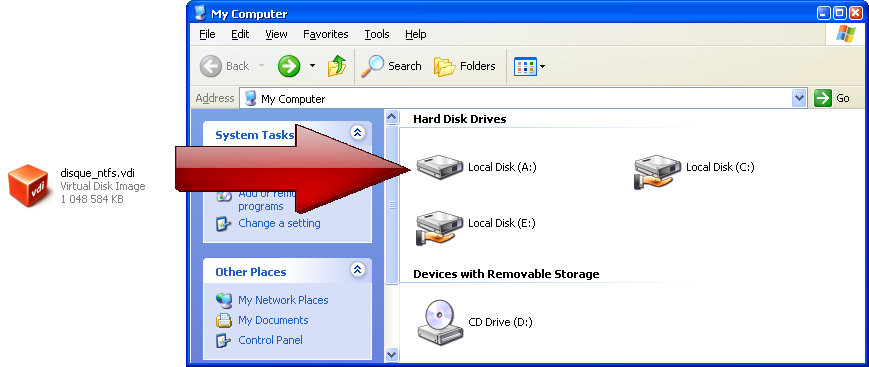
\includegraphics[scale=0.45]{images/Montage_Windows.png}
	\caption{Montage d'un disque virtuel dans la machine hôte (Windows)}
	\label{Montage Windows}
\end{figure}

Le disque virtuel permet, grâce à l'hyperviseur, d'émuler un disque dur (ou une clé USB).
Comme expliqué dans la partie \ref{Particularités de la virtualisation}, ils peuvent être branchés ou débranchés de la machine virtuelle comme s'ils étaient de vrais disques durs.

Mais il est aussi possible d'utiliser ce disque virtuel de la même manière sur la machine hôte Windows.
Il existe des outils qui permettent de monter ce disque virtuel pour qu'il apparaisse en tant que nouveau volume, dans l'interface du "Poste de travail".
Cela permet ainsi de parcourir les fichiers, de les modifier, et même de formater le disque comme s'il s'agissait d'un vrai disque dur.
\\



%%%%%%%%%%%%%%%%%%%%%%%%%%%%%%%%%%%%%%%%%%%%%%%%%%%%%%%%%%%%%%%%%%%%%%%%%%%%%%%%%%%%%%%%%%%%%%%%%%%%

\subsubsection{imDisk}

\begin{figure}[!h]
	\center
	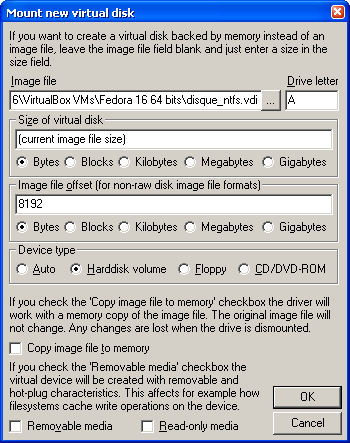
\includegraphics[scale=0.5]{images/imDisk.png}
	\caption{Interface graphique de imDisk}
	\label{Interface graphique de imDisk}
\end{figure}

Pour ce faire, j'utiliserai \textit{imDisk}\footnote{imDisk - Lien : \href{http://www.ltr-data.se/opencode.html/\#ImDisk}{http://www.ltr-data.se/opencode.html/\#ImDisk}} qui est gratuit et open-source.
Ce programme dispose d'une interface graphique (capture d'écran \ref{Interface graphique de imDisk}), mais est aussi utilisable en ligne de commande.
\\


Pour monter un disque virtuel sur Windows il est nécessaire de spécifier un \textit{offset}.
Cet offset correspond à la taille des données situées en en-tête du fichier (confère la partie \ref{Les disques virtuels} qui détaille la structure d'un disque virtuel).
Ainsi le programme accèdera directement au disque encapsulé. 
\\



%%%%%%%%%%%%%%%%%%%%%%%%%%%%%%%%%%%%%%%%%%%%%%%%%%%%%%%%%%%%%%%%%%%%%%%%%%%%%%%%%%%%%%%%%%%%%%%%%%%%

\subsubsection{Principe de l'échange}

L'échange de fichier peut donc s'effectuer par l'intermédiaire d'un disque virtuel de la même manière que l'on échangerait un fichier entre deux ordinateurs à l'aide d'une clé USB :
\begin{enumerate}
	\item monter le disque virtuel sur la machine hôte (Windows) ;
	\item copier les fichiers sources sur le volume ;
	\item démonter le disque virtuel de la machine hôte ;
	\item brancher puis monter le disque virtuel dans la machine virtuelle (Linux) ;
	\item copier les fichiers vers le répertoire cible ;
	\item démonter puis débrancher le disque virtuel de la machine virtuelle.
\end{enumerate}
Pour la réception de fichiers le principe est exactement le même mais en copiant d'abord la source dans la machine virtuelle avant d'effectuer la copie dans la machine hôte.
\\



%%%%%%%%%%%%%%%%%%%%%%%%%%%%%%%%%%%%%%%%%%%%%%%%%%%%%%%%%%%%%%%%%%%%%%%%%%%%%%%%%%%%%%%%%%%%%%%%%%%%

\subsubsection{Inconvénients}
\label{Inconvénients de l'échange par disque virtuel}

Cette solution fonctionne, mais pose plusieurs problèmes :
\begin{itemize}
	\item Cela demande de nombreuses opérations qui sont susceptibles d'échouer : disque virtuel inexistant, corrompu ou de trop petite taille, échec du branchement, débranchement du disque alors que la copie n'est pas terminée, \ldots
	\item Ensuite, chacune de ces opérations peut durer quelques secondes.
Par exemple lorsque l'on branche un disque virtuel sur la machine virtuelle (Linux), celle-ci ne le reconnait pas instantanément et il faut attendre environ 2 secondes.
	\item Enfin l'échange impose d'effectuer la copie deux fois : une première fois sur le disque virtuel, et une seconde fois dans la machine virtuelle (si envoi) ou hôte (si réception).
\\
\end{itemize}




%%%%%%%%%%%%%%%%%%%%%%%%%%%%%%%%%%%%%%%%%%%%%%%%%%%%%%%%%%%%%%%%%%%%%%%%%%%%%%%%%%%%%%%%%%%%%%%%%%%%
%%%%%%%%%%%%%%%%%%%%%%%%%%%%%%%%%%%%%%%%%%%%%%%%%%%%%%%%%%%%%%%%%%%%%%%%%%%%%%%%%%%%%%%%%%%%%%%%%%%%
%%%%%%%%%%%%%%%%%%%%%%%%%%%%%%%%%%%%%%%%%%%%%%%%%%%%%%%%%%%%%%%%%%%%%%%%%%%%%%%%%%%%%%%%%%%%%%%%%%%%

\subsection{Comparaison}
\label{Comparaison}

Deux types de calcules sont généralement effectués sur les outils scientifiques :
\begin{itemize}
	\item Le calcul intensif qui s'effectue sur un fichier d'entrée volumineux pouvant atteindre 1Go ;	
	\item Le plan d'expérience qui s'effectue quant à lui sur une multitude de petits fichiers d'entrée.
\end{itemize}

Pour pouvoir comparer ces différentes solutions, j'ai étudié la rapidité de l'échange en faisant varier le nombre de fichiers, ainsi que leur taille.
\\



%%%%%%%%%%%%%%%%%%%%%%%%%%%%%%%%%%%%%%%%%%%%%%%%%%%%%%%%%%%%%%%%%%%%%%%%%%%%%%%%%%%%%%%%%%%%%%%%%%%%

\subsubsection{Conditions des tests}

Pour ne pas influencer les résultats, ni la machine hôte ni la machine virtuelle n'ont été utilisées lors des différents tests.
La fonction \lstinline{time.time()} a été introduite dans les méthodes d'échange, permettant d'obtenir l'heure courant, et donc obtenir la durée de l'échange par différence.
Les résultats sont obtenus en calculant la moyenne sur un échantillon de 5 échanges, le nombre de fichier varie entre 1 et 10.000, et la taille du fichier varie entre 1ko et 1Go.
\\



%%%%%%%%%%%%%%%%%%%%%%%%%%%%%%%%%%%%%%%%%%%%%%%%%%%%%%%%%%%%%%%%%%%%%%%%%%%%%%%%%%%%%%%%%%%%%%%%%%%%

\subsubsection{Résultats obtenus : analyse et critique}

\begin{figure}[!h]
	\center
	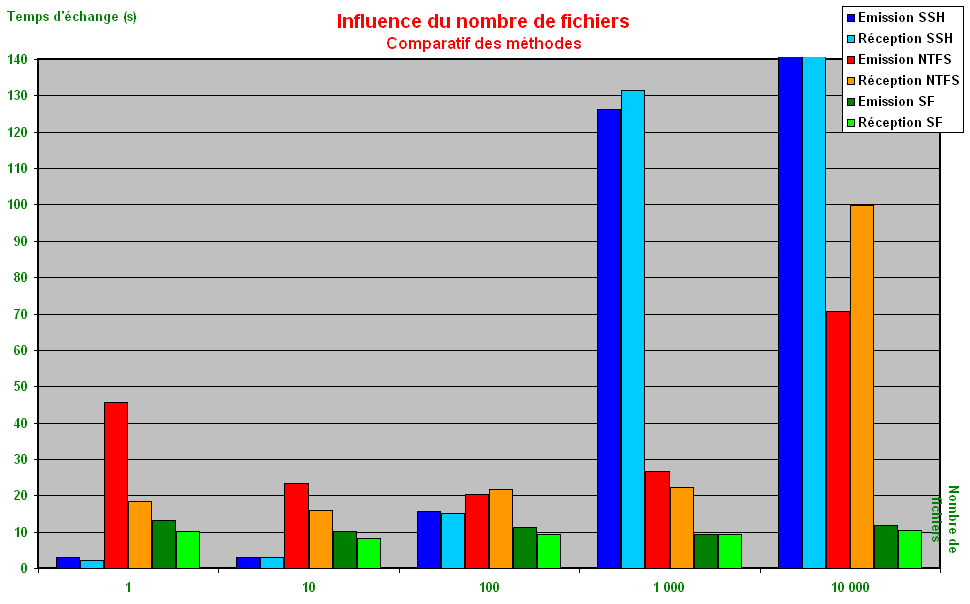
\includegraphics[scale=0.45]{images/tests/nombre_comparatif.png}
	\caption{Temps d'échange en fonction du nombre de fichiers}
	\label{temps=f(nombre) - comparatif}
\end{figure}

\begin{figure}[!h]
	\center
	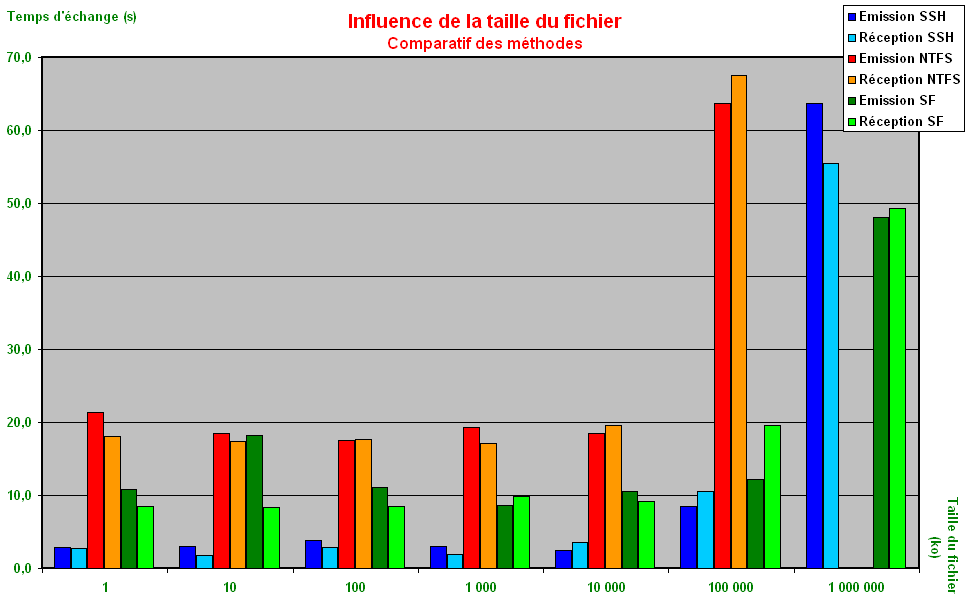
\includegraphics[scale=0.45]{images/tests/taille_comparatif.png}
	\caption{Temps d'échange fonction de la taille du fichier}
	\label{temps=f(taille) - comparatif}
\end{figure}

Notons que l'axe des ordonnées se limite à 140 secondes, mais le temps d'échange avec la méthode SSH atteint 1250 secondes pour 10.000 fichiers.
Les résultats sont reportés dans un tableau en annexe.
\\


\paragraph{SSH :}
On peut remarquer que le temps d'échange est "plus ou moins" proportionnel au nombre de fichier.
De plus, le temps d'échange est relativement faible et constant, pour des fichiers de taille inférieure à 10Mo et pour un ensemble de 100 fichiers.


\paragraph{Disque virtuel :}
Le graphique "Étude de la méthode NTFS" présent en annexe détaille les différentes étapes de l'échange.
La durée notée "Autre" correspond aux étapes de (dé)branchement et (dé)montage du disque virtuel dans la machine virtuelle et la machine hôte.
Ce temps est constant car les fichiers n'ont aucune influence sur ces actions.

On remarque que les inconvénients présentés dans la partie \ref{Inconvénients de l'échange par disque virtuel} sont bien présents :
\begin{itemize}
	\item la durée des deux copies est globalement très faible et constante, mais se fait doublement ressentir lors de la réception de 10.000 fichier ou d'un fichier de 100Mo,
	\item la durée de l'échange est très élevée pour les fichiers de petite taille et en petit nombre,
	\item un problème survient lors de la copie d'un fichier d'1Go sur le disque virtuel monté dans Windows, apparemment lors du "flush du buffeur".
\end{itemize}


\paragraph{Répertoire partagé :}
Le graphique "Étude de la méthode SF" présent en annexe détaille les différentes étapes de l'échange.
La durée notée "Autre" correspond aux étapes de partage du répertoire et de (dé)montage du répertoire partagé dans la machine virtuelle.
De même que pour le disque virtuel, la durée est constante car les fichiers n'ont pas d'influence sur les actions.

Cette méthode est globalement la plus performante, car le temps de l'échange est constant quelque soit le nombre et la taille des fichiers, à l'exception du fichier de 1Go où la durée de l'échange atteint raisonnablement les 50 secondes.

Il serait possible d'améliorer le temps noté "Autre" en développant un script qui monterait et effectuerait la copie (étape 2 et 3), plutôt que d'exécuter les deux commandes séparément (confère la partie \ref{Principe de l'échange par répertoire partagé} pour plus de détails).
Cette technique est évoquée dans la partie \ref{Utilisation de PLink} pour diminuer fortement le temps d'exécution en lançant plusieurs commandes simultanément avec PLink.
\\



%%%%%%%%%%%%%%%%%%%%%%%%%%%%%%%%%%%%%%%%%%%%%%%%%%%%%%%%%%%%%%%%%%%%%%%%%%%%%%%%%%%%%%%%%%%%%%%%%%%%

\subsubsection{Conclusion}

Pour des raisons de simplicité de programmation et d'utilisation j'utiliserai la méthode SSH dans la première version de ma solution, qui permet un temps de transfert assez rapide pour des fichiers de taille et quantités raisonnables.

La solution qui pourrait être utilisée dans les prochaines versions serait d'effectuer un test sur la source à échanger.
Par exemple si le nombre ou la taille des fichiers à échange est faible on utilisera la méthode SSH, et pour les gros ou nombreux fichiers on utilisera le répertoire partagé.
